\section{Diagnostic set B: matched calibration memory}
\label{sec:matchedsupp}
The matched-memory follow-up contains ten additional spline replays: two captures and seeds 42--46. Its protocol and runner were committed before their full executions, after the earlier results and concerns about unequal calibration memory had been examined. It is exploratory on both captures. The larger disjoint ROLE256 buffer receives the same CAL-role arrivals as ROLE64, preserves the original class-eviction rule with borrowing of unused slots, and applies the same 50-block age filter. Occurrence-level nesting of the small buffer inside the large one and FIT/CAL digest disjointness are checked at every arrival. All four thresholds use the successful original FIT192/ROLE64 transaction gate, so the score trajectory and its timing are identical across calibration capacities.

\begin{figure}[tb]
\centering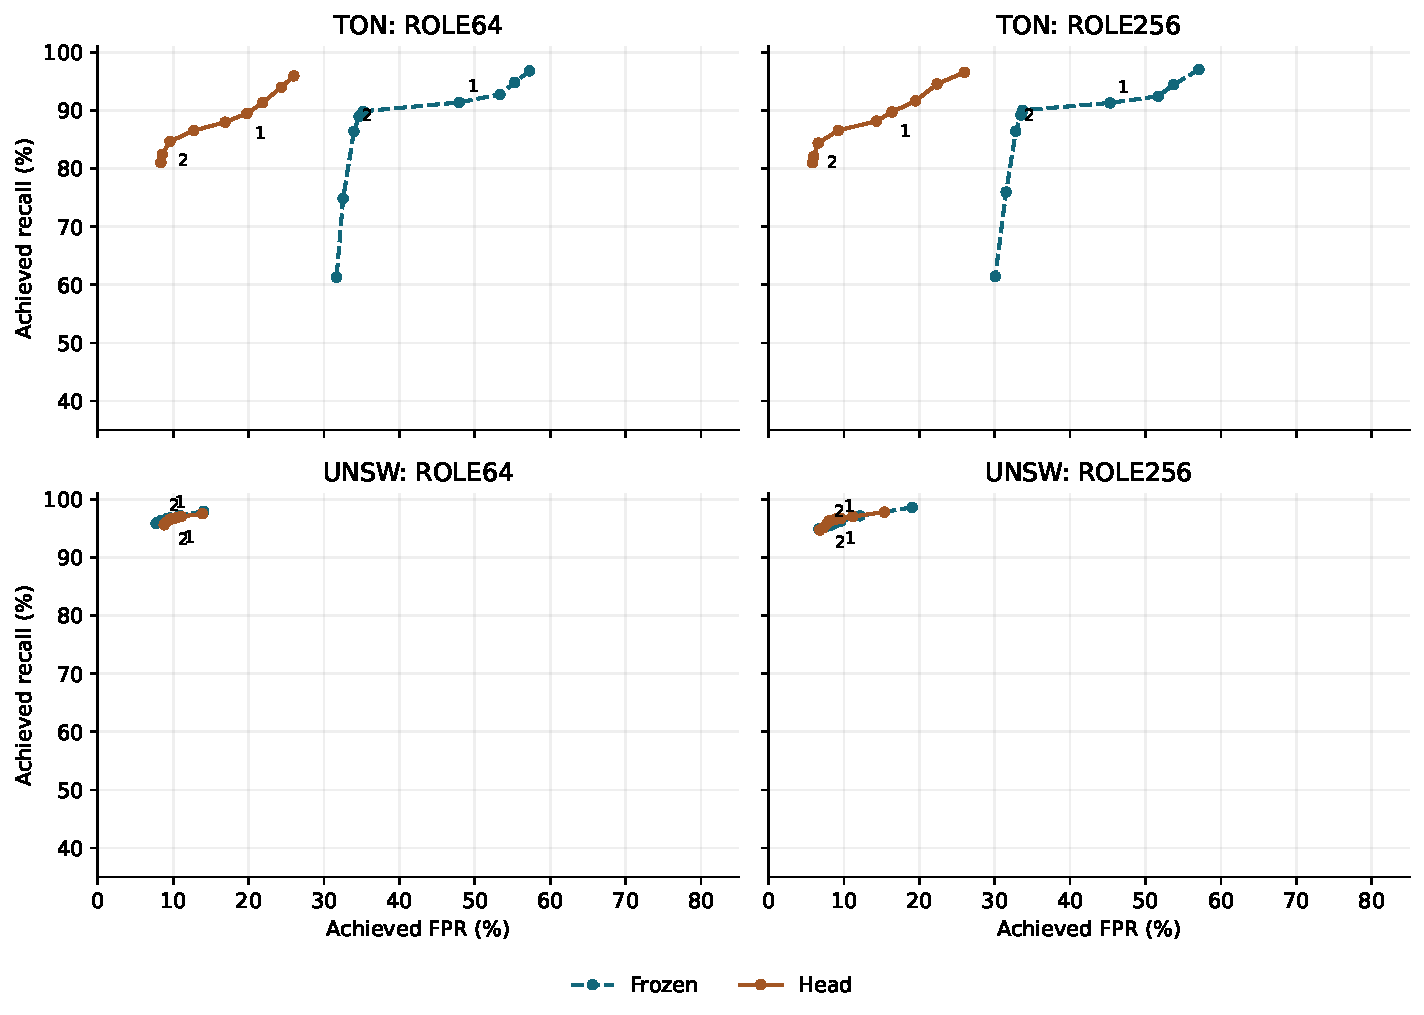
\includegraphics[width=.94\linewidth]{figures/diagnostic_b_same_memory.pdf}
\caption{Same-memory score comparisons, with identical axes in all panels. Within a panel, frozen and head scores use the same calibration occurrences and update times; the head trajectory also stays fixed across columns. The nine cost weights generate causal operating policies, connected in cost-weight order. Numerals mark $\lambda=1$ and 2. Points are means across five randomizations conditional on one capture, not a deployable oracle frontier.}
\Description{Same-memory score comparisons, with identical axes in all panels. Within a panel, frozen and head scores use the same calibration occurrences and update times; the head trajectory also stays fixed across columns. The nine cost weights generate causal operating policies, connected in cost-weight order. Numerals mark $\lambda=1$ and 2. Points are means across five randomizations conditional on one capture, not a deployable oracle frontier.}
\end{figure}

\begin{table}[tb]
\centering\fontsize{9}{10.5}\selectfont\setlength{\tabcolsep}{2.4pt}
\caption{FPR targets with matched CAL-role memory and update times. All entries are percentages, mean $\pm$ conditional seed SD. Target is a requested calibration rate; future FPR is measured separately. CAL denotes capacity, not the number of eligible observations at every update.}
\begin{tabular}{lrr rrr rrr}\toprule
& & & \multicolumn{3}{c}{Frozen score} & \multicolumn{3}{c}{Head score}\\
Stream & CAL & Target & Recall & FPR & BA & Recall & FPR & BA\\\midrule
\tablerows{tables/diagnostic_b_target_rows.tex}
\bottomrule\end{tabular}
\end{table}

For TON, the cost-weight polylines of the matched-memory frozen and head controllers have no paired common support at the prespecified 10\%, 13\%, or 20\% FPR targets. Their corresponding matched-error estimates are therefore missing, rather than extrapolated. At 10\% FPR on UNSW, five pairs are supported at both capacities: head-minus-frozen recall is $-0.21\pm0.27$ points at ROLE64 and $+0.36\pm0.30$ at ROLE256. At 13\%, only three ROLE64 pairs and all five ROLE256 pairs are supported. These are descriptive interpolations of the recorded cost policies. They must not be substituted for the original all-label-control interpolation or the causal FPR-target controllers.

The report set includes every per-block confusion matrix for all, seen, and unseen observations, head-state digests, thresholds, request digests, CAL class counts and age ranges, and update-gate outcomes. Every shared trajectory agrees exactly with the retained second diagnostic run. The executable source, parent reports, inputs and initial fitted states are identified by SHA-256. The initial setup attempts failed on an audit-file path and an overly strict assertion that treated soft eviction quotas as hard class maxima; neither produced a complete result report or changed the experimental design. The final runner checks the original borrowing rule and records 274,090 replay checks. A separate analysis verifies source hashes and recomputes every aggregate from the block counts (1,930 checks).

\subsection{Role salts and within-setting randomization}
\begin{table}[!htbp]
\centering\small
\caption{Default Head/ROLE64 at $\lambda=1$ for each of three fixed role salts. Means and sample SDs are over five seeds conditional on that salt and the single capture. These rows repeat the earlier sensitivity evidence in a form that separates salt choice from within-salt variation.}
\begin{tabular}{llrrr}\toprule
Stream & Role salt & Recall & FPR & BA\\\midrule
\tablerows{tables/diagnostic_b_salt_rows.tex}
\bottomrule\end{tabular}
\end{table}
The three role salts span 5.02 BA points on TON and 3.59 points on UNSW. These are sensitivities to declared deterministic partitions, not confidence bounds for a salt distribution. Memory size, age and minimum-count interventions change other controller components and are reported separately. Neither type of sensitivity is an independent replication of a capture.
